\usetikzlibrary{positioning,matrix,fit}
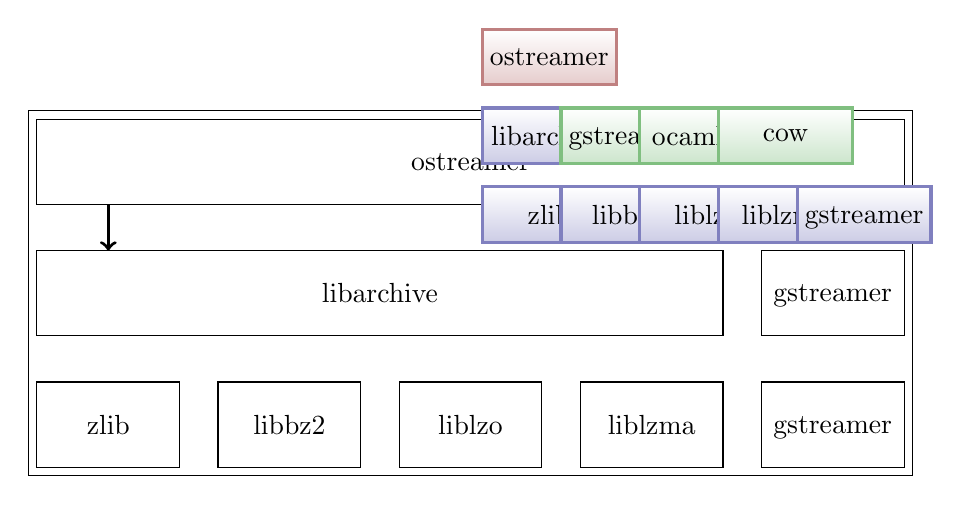
\begin{tikzpicture}[
  redblock/.style={
    rectangle,
    very thick,
    draw=red!50!black!50,
    top color=white,
    bottom color=red!50!black!20,
    inner sep=0em,
    minimum width=17mm,
    minimum height=2em
  },
 blueblock/.style={
    rectangle,
    very thick,
    draw=blue!50!black!50,
    top color=white,
    bottom color=blue!50!black!20,
    inner sep=0em,
    minimum width=17mm,
    minimum height=2em,
    text depth=0
  },
 greenblock/.style={
    rectangle,
    very thick,
    draw=green!50!black!50,
    top color=white,
    bottom color=green!50!black!20,
    inner sep=0em,
    minimum width=17mm,
    minimum height=2em,
    text depth=0
  },
  testblock/.style={draw,inner sep=0mm}]
      \matrix (table) [%
        minimum width = 18mm,
        draw,
        matrix of nodes,
        nodes in empty cells,
        row  sep=6mm,column sep=5mm
        ]{
  & & & & \\
  & & & & \\
  & & & & \\
  & & & & \\
  & & & & \\
  & & & & \\
 };
  \node [testblock,fit=(table-1-1)(table-2-5),label={center:ostreamer}] {};
  % level 2
  \node [testblock,fit=(table-3-1)(table-4-4),label={center:libarchive}] {};
  \node [testblock,fit=(table-3-5)(table-4-5),label={[text depth=0]center:gstreamer}]
 {};
 % level 3
  \node [testblock,fit=(table-5-1)(table-6-1),label={center:zlib}] {};
  \node [testblock,fit=(table-5-2)(table-6-2),label={center:libbz2}] {};
  \node [testblock,fit=(table-5-3)(table-6-3),label={center:liblzo}] {};
  \node [testblock,fit=(table-5-4)(table-6-4),label={center:liblzma}] {};
  \node [testblock,fit=(table-5-5)(table-6-5),label={[text depth=0]center:gstreamer}] {};
  \begin{scope}
  \draw[->,very thick] (table-2-1) -- (table-3-1);
  \end{scope}

  \draw (1,3) node[redblock] {ostreamer};
  \draw (1,2) node[blueblock] {libarchive};
  \draw (2,2) node[greenblock] {gstreamer};
  \draw (3,2) node[greenblock] {ocamlnet};
  \draw (4,2) node[greenblock] {cow};
  \draw (1,1) node[blueblock] {zlib};
  \draw (2,1) node[blueblock] {libbz2};
  \draw (3,1) node[blueblock] {liblzo};
  \draw (4,1) node[blueblock] {liblzma};
  \draw (5,1) node[blueblock] {gstreamer};

\end{tikzpicture}
% http://tex.stackexchange.com/questions/94343/matrix-of-nodes-over-multiple-columns-in-tikz